\documentclass[11pt]{article}
\usepackage{geometry}                
\geometry{letterpaper}                 
\usepackage[parfill]{parskip}        
\usepackage{graphicx}
\usepackage{amssymb}
\usepackage{amsmath}
\usepackage{epstopdf}
\usepackage{verbatim}
\usepackage{float}
\usepackage{enumerate}
\usepackage{hyperref}
\usepackage[utf8]{inputenc}
\usepackage[T1]{fontenc}
\DeclareGraphicsRule{.tif}{png}{.png}{`convert #1 `dirname #1`/`basename #1 .tif`.png}
\usepackage{color}
\usepackage{textcomp}
\definecolor{listinggray}{gray}{0.9}
\definecolor{lbcolor}{rgb}{1,1,1}

\begin{document}
{\small
\section*{Problems for Discussion 4, 10/02/13}
Compiled by Mai Le, some problems from Prof. Fessler, Prof. Yagle, and O\&W
}
\section{Inverse Z-Transform}
% Yagle, disc 4, #4
$X(z) = \frac{2z^2-1.5z}{z^2-1.5z+0.5}$

Determine the three possible ROCs of this z-transform and the corresponding time-domain sequences (inverse z-transforms).

%{\color{blue}
%$\frac{X(z)}{z} = \frac{\frac{2z^2-1.5z}{z^2-1.5z+0.5}}{z} = \frac{2z-\frac{3}{2}}{(z-\frac{1}{2})(z-1)} = \frac{A_1}{z-\frac{1}{2}}+\frac{A_2}{z-1}$
%
%$A_1 = \frac{X(z)}{z}\left(z-\frac{1}{2}\right)\bigg|_{z=\frac{1}{2}}=\frac{2z-\frac{3}{2}}{z(z-1)}\bigg|{z=\frac{1}{2}}=\frac{-\frac{1}{2}}{-\frac{1}{4}} = 2$
%
%$A_2 = \frac{X(z)}{z}\left(z-1 \right)\bigg|_{z=1} = \frac{2z-\frac{3}{2}}{z(z-\frac{1}{2}}\bigg|{z=1} = \frac{\frac{1}{2}}{\frac{1}{2}} = 1 $
%
%$\frac{X(z)}{z} = \frac{2}{z-\frac{1}{2}}+\frac{1}{z-1} $
%
%$X(z) = \frac{2z}{z-\frac{1}{2}}+\frac{z}{z-1} $
%
%\begin{enumerate}
%	\item ROC: $|z|<\frac{1}{2}$ \\
%	\qquad $x[n]=-2\left(\frac{1}{2}\right)^n u[-n-1]-u[-n-1]$.
%	\item ROC: $\frac{1}{2}<|z|<1$ \\
%	\qquad $x[n]=2\left(\frac{1}{2}\right)^n u[n] - u[-n-1]$
%	\item ROC: $|z|>1$ \\
%	\qquad $x[n]=2\left(\frac{1}{2}\right)^nu[n]+u[n]$
%\end{enumerate}
%}

\section{All zeros and all poles}
% from Fessler notes, p. 3.15

If $X(z)$ has the form $X(z)=\sum\limits_{k=0}^M b_k z^{-k}=\frac{1}{z^M}\sum\limits_{k=0}^M b_kz^{M-k}=\frac{\prod_{k=1}^M (z-z_k)}{z^M}$, then what can we say about the poles and zeros? What can we say about the duration of $x[n]$?

%{\color{blue}
%The $M$ poles at $z=0$ are called trivial poles. They correspond only to a time shift. 
%
%There are $M$ roots of the numerator that are nontrivial zeros. This is an "all-zero system".
%
%The time-domain sequence has finite duration: $x[n]=\sum\limits_{k=0}^N b_k \delta[n-k]$.
%}
%
If $X(z)$ has the form $X(z)=\frac{b_0}{1+\sum\limits_{k=1}^N a_k z^{-k}}=\frac{b_0 z^N}{\sum\limits_{k=0}^N a_k z^{N-k}} = b_0 \frac{z^N}{\prod_{k=1}^N (z-p_k)}$, then what can we say about the poles and zeros? What can we say about the duration of $x[n]$?

%{\color{blue}
%The $N$ poles at $z=0$ are trivial zeros. The denominator polynomial has $N$ roots that are poles, thus this is called an "all-pole system". 
%
%The time-domain sequence has infinite duration.
%}
{\color{red}
This problem was intended to be a fun theoretical exploration of the effect of poles and zeros. However, I'm cutting it from the list because it generated more confusion than understanding. I also want to emphasize that this type of analysis is not expected in the exam. If you are curious about this topic, talk to me in office hours, or wait until we discuss system response functions formally in lecture. Sorry for the mess!

}

\section{ROCs and Convolution}
% from Fessler notes, p. 3.8

Let $h[n]=\delta[n]-\delta[n-1]$ (discrete-time differentiator), $x[n]=u[n-2]$, and $y[n]=x[n]*h[n]$. What is the ROC of $Y(z)$?

%{\color{blue}
%$H(z) = 1-z^{-1}$ with $ROC_H$: $z \neq 0$.
%
%$X(z) = \frac{z^{-2}}{1-z^{-1}}$ with $ROC_X$: $|z|>1$.
%
%Since $y[n]=x[n]*h[n]$, so $Y(z)=H(z)X(z)=\left(1-z^{-1} \right)\left( \frac{z^{-2}}{1-z^{-1}} \right) = z^{-2}$ which has ROC $z \neq 0$. Note that this ROC is bigger than the intersection of $ROC_X$ and $ROC_H$.
%
%$y[n] = u[n-2]* \left(\delta[n]-\delta[n-1]\right) \delta[n-2]$ is a finite duration sequence, so it will converges over all values of $z$, except possibly $z=0$ or $z=\infty$. In this case, $y[n]$ converges for $z=\infty$ but not $z=0$.
%}

\section{Causality and Pole-Zero Plots}
% Fessler notes 3.32
One of the following pole-zero plots corresponds to a causal system. Which one?

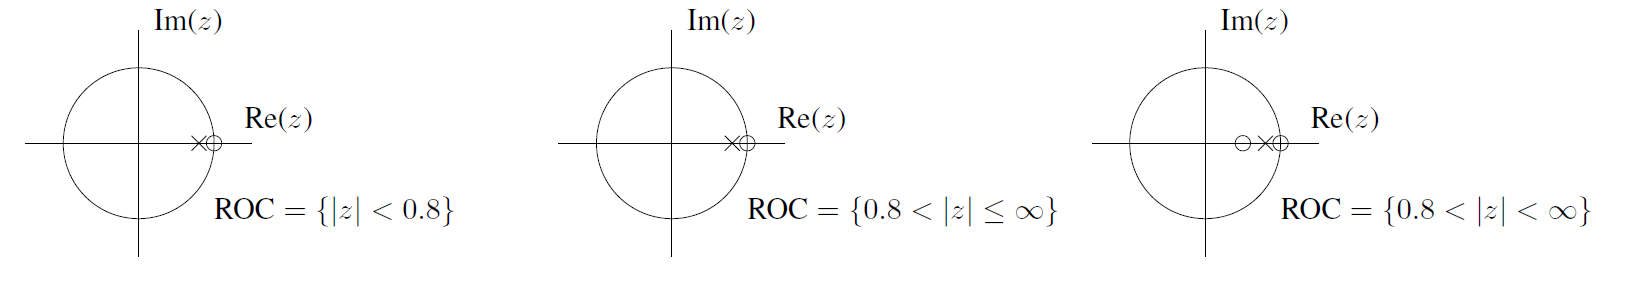
\includegraphics[width=\textwidth]{causal_pole_zero_plots.png} 

%{ \color{blue}
%Only the middle pole-zero plot corresponds to a causal system. For the left one, the ROC extends inward, which is only true for left-sided sequences. For the right one, $H(z) = g \frac{(z-1)(z-\frac{1}{2})}{z-0.8}$ (we don't know the scaling factor $g$) which is infinite at $z=\infty$, so it is noncausal. For further explanation why $X(\infty)<\infty$ for causal $x[n]$, see solution below for "Causality and the Z-Transform".
%
%}

\section{Causality and the Z-Transform}
% O&S 3.11 in 2nd ed. (also 3.11 in 3rd ed.)
Which of the following could be the z-transform of a causal sequence? Do not evaluate the inverse transform. You should be able to give the answer by inspection.

%{\color{blue}
%$x[n]$ is causal, so $X(z)=\sum\limits_{n=0}^\infty x[n] z^{-n}$. Therefore the summation will include no positive powers of $z$. Thus, $X(z)$ must converge at $z=\infty$ (i.e. $z=\infty$ must be in the ROC, $\lim_{z\rightarrow \infty} X(z) \neq \infty$
%}

\subsection*{(a) $\frac{(1-z^{-1})^2}{(1-\frac{1}{2}z^{-1})}$}

%{\color{blue}
%$\lim_{z\rightarrow \infty} \frac{(1-z^{-1})^2}{(1-\frac{1}{2}z^{-1})} = \lim_{z\rightarrow \infty} \frac{z^2-2z+1}{z^2-\frac{1}{2}z} = 1$, could be causal
%}

\subsection*{(b) $\frac{(z-1)^2}{(z-\frac{1}{2})}$}

%{\color{blue}
%$\lim_{z\rightarrow \infty} \frac{(z-1)^2}{(z-\frac{1}{2})} = \lim_{z\rightarrow \infty} \frac{z^2-2z+1}{z-\frac{1}{2}} = \infty$, could not be causal
%}

\subsection*{(c) $ \frac{(z-\frac{1}{4})^5}{(z-\frac{1}{2})^6}$}

%{\color{blue}
%$\lim_{z\rightarrow \infty} \frac{(z-\frac{1}{4})^5}{(z-\frac{1}{2})^6} = 0$, could be causal
%}

\subsection*{(d) $ \frac{(z-\frac{1}{4})^6}{(z-\frac{1}{2})^5}$}

%{\color{blue}
%$\lim_{z\rightarrow \infty} \frac{(z-\frac{1}{4})^6}{(z-\frac{1}{2})^5} = \infty$, could not  be causal
%}

\section{Z-Transform Deduction}
% O&W 10.31
We are given the following facts about a discrete-time signal $x[n]$ with z-transform $X(z)$:
\begin{enumerate}
	\item $X(z)$ can be written as a ratio of polynomials in $z$.
	\item $x[n]$ is real and right-sided
	\item $X(z)$ has exactly 2 poles.
	\item $X(z)$ has two zeros at the origin and no other zeros.
	\item $X(z)$ has a pole at $z=\frac{1}{2}e^{j \pi /3}$
	\item $X(1)=\frac{8}{3}$
\end{enumerate}
Determine $X(z)$ and its region of convergence.  

%{\color{blue}
%
%Our goal is to determine $X(z)$ and its ROC. From facts 2 and 3, we know that $X(z)$ has the following form:
%
%\begin{equation*}
%X(z) = a \frac{z^2}{(z-p_1)(z-p_2)}
%\end{equation*}
%
%where $p_1$ and $p_2$ are the two poles. Since we have two zeros at the origin, we have a numerator of $z^2$, but with a possible scaling factor $a$.
%
%Since we are told in fact 4 one of the pole values, let's plug it in.
%
%\begin{equation*}
%X(z) = a \frac{z^2}{(z-\frac{1}{2}e^{j \pi /3})(z-p_2)}
%\end{equation*}
%
%Because $x[n]$ is real (fact 1) and from the complex conjugate root theorem, we know that roots of the denominator must either be real or part of a complex conjugate pair. Thus, the other pole has to be $\frac{1}{2}e^{-j\pi/3}$.
%
%\begin{equation*}
%X(z) = a \frac{z^2}{(z-\frac{1}{2}e^{j \pi /3})(z-\frac{1}{2}e^{-j\pi/3})}
%\end{equation*}
%
%Now to find the scaling factor $a$, let us evaluate $X(z=1)$ and compare with the value given in fact 5.
%
%$X(1) = a \frac{1^2}{(1-\frac{1}{2}e^{j \pi /3})(1-\frac{1}{2}e^{-j\pi/3})} = \frac{a}{1-\frac{1}{2}e^{j \pi /3}-\frac{1}{2}e^{-j \pi /3}+\frac{1}{4}} = \frac{a}{\frac{5}{4}-cos(\pi/3)} = \frac{a}{\frac{5}{4}-\frac{1}{2}}=\frac{4}{3}a$
%
%Since we need $\frac{4}{3}a = \frac{8}{3}$, we choose $a=2$. This gives us a final form for $X(z)$.
%
%\begin{equation*}
%X(z) = 2 \frac{z^2}{(z-\frac{1}{2}e^{j \pi /3})(z-\frac{1}{2}e^{-j\pi/3})}
%\end{equation*}
%
%Now, to deduce the ROC of $X(z)$, we use the right-sidedness of $x[n]$, given in fact 1, along with ROC property \#5, to say that the ROC extends outward from the outermost pole. In this case, both $\frac{1}{2}e^{j \pi /3}$ and $\frac{1}{2}e^{-j \pi /3}$ tie as the outermost poles, with magnitudes of $\frac{1}{2}$. So ROC $=\{|z|>\frac{1}{2}\}$. 
%
%This also makes sense because fact 5 tells us that the ROC converges for $z=1$, so the unit circle must be in the ROC. This agrees with our answer.
%}

\section{Inverse Z-Transform with Multiple Poles at Origin}
% Yagle lecture notes izxform, Ex #3

Consider $X(z) = \frac{z^3+2z^2+3z+4}{z^2(z-1)}$. Use the "convolution in time is multiplication in z" theorem to find a right-sided $x[n]$.

%{\color{blue}
%$X(z) = \frac{z^3+2x^2+3z+4}{z^2(z-1)} =\frac{z^3+2z^2+3z+4}{z^3}\frac{z}{z-1}=\underbrace{\left(1+2z^{-1}+3z^{-2}+4z^{-3}\right)}_{A(z)} \underbrace{\frac{z}{z-1}}_{B(z)}$
%
%So, $x[n]=a[n]*b[n] = \{\underline{1},2,3,4\}*u[n]= u[n]+2u[n-1]+3u[n-2]+4u[n-3]$.
%
%For more detail on the last step, $\{\underline{1},2,3,4\} = \delta[n]+2\delta[n-1]+3\delta[n-2]+4\delta[n-3]$. From the distributivity of convolution, we have $\left(\delta[n]+2\delta[n-1]+3\delta[n-2]+4\delta[n-3] \right)*u[n] = \delta[n]*u[n]+2\delta[n-1]*u[n]+3\delta[n-2]*u[n]+4\delta[n-3]*u[n]$. Since convolving any function with a shifted delta results in the original function being shifted, we arrive at $x[n] = u[n]+2u[n-1]+3u[n-2]+4u[n-3]$.
%
%}

\end{document}